\documentclass[10pt,a4paper]{article}
\usepackage[utf8]{inputenc}
\usepackage[german]{babel}
\usepackage{mathrsfs}
\usepackage{amsmath}
\usepackage{amsfonts}
\usepackage{amssymb}
\usepackage{amsthm}
\usepackage[left=2cm,right=2cm,top=2cm,bottom=2cm]{geometry}
\usepackage{minted}
\usepackage{graphicx}

\begin{document}

\section{Aufgabe 1}

\subsection{Teil a}

The first thing to note, is that all inner sums are always $\ge 0$. Now examine
an inner sum
\begin{equation}
  \sum_{i} z_{i}^{n} ||x_{n} - \mu_{i}||^{2} = ||x_{n} - \mu_{j}||^{2}
\end{equation}
for some $j \in \{ 1, \dots, k \}$, because every $z^{n}$ has only one $1$
entry. After updating $z$ the new value of the inner sum is
\begin{equation}
  \sum_{i} z_{i}^{n} ||x_{n} - \mu_{i}||^{2} = ||x_{n} - \mu_{k}||^{2}
\end{equation}
for $k = \arg\,\min_{j} ||x_{n} - \mu_{j}||^{2}$. So the updated inner sum is
the minimum over all $\mu$ and such always less than or equal to all other
possible terms. So every inner sum decreases after updating, so their sum does,
too.

\subsection{Teil b}

\begin{equation}
  J = \sum_{i = 1}^{n} \sum_{j = 1}^{k} z_{j}^{i} (x_{i} - \mu_{j})^{T}(x_{i} - \mu_{j})
\end{equation}
Now take the differential with respect to $\mu_{g}$ for $g \in \{ 1, \dots, k \}$.
\begin{equation}
  d_{\mu_{g}} \sum_{i = 1}^{n} \sum_{j = 1}^{k} z_{j}^{i} (x_{i} - \mu_{j})^{T}(x_{i} - \mu_{j}) = -2 \sum_{i = 1}^{n} z_{g}^{i} (x_{i} - \mu_{g})^{T}d_{\mu_{g}}\mu_{g}
\end{equation}
Set it to zero.
\begin{equation}
  -2 \sum_{i = 1}^{n} z_{g}^{i} (x_{i} - \mu_{g})^{T} = 0 \Leftrightarrow -2 \sum_{i = 1}^{n} z_{g}^{i} x_{i}^{T} + 2 \sum_{i = 1}^{n} z_{g}^{i} \mu_{g}^{T} = 0 \Leftrightarrow 2 \mu_{g}^{T} \sum_{i = 1}^{n} z_{g}^{i} = 2 \sum_{i = 1}^{n} z_{g}^{i} x_{i}^{T} \Leftrightarrow \mu_{g}^{T} = \frac{\sum_{i = 1}^{n} z_{g}^{i} x_{i}^{T}}{\sum_{i = 1}^{n} z_{g}^{i}}
\end{equation}
The equation can be transposed, so we have an extremum at
\begin{equation}
  \mu_{g} = \frac{\sum_{i = 1}^{n} z_{g}^{i} x_{i}}{\sum_{i = 1}^{n} z_{g}^{i}}
\end{equation}
Now one can argue, that this must be a minimum, because it is the only extremum
and surely we can make $J$ arbitrarily large by adding an arbitrary nonzero
vector onto $\mu_{g}$, so $J$ tends to infinity in every direction.

\subsection{Teil c}

The conclusion from the first two parts is, that $J^{(i)}$ is a decreasing
sequence, where $i$ is the iteration of the algorithm. And as $J^{(i)}$ is
bounded from below by $0$, it converges. So k-means converges towards a state,
that minimizes the distortion measure.

\section{Aufgabe 2}

\begin{minted}{julia}
using Gadfly, Distributions

# Number of clusters
k = 2

# True means
mus = [[-1, -1] [1, 1]]
# Random cluster centers
#mus = rand(2, k)

# Sample test data from the clusters
sigma2 = 1 / 2
Sigma = sigma2 * eye(2, 2)
numPoints = 40
data = [rand(MvNormal(float(mus[:, i]), Sigma), numPoints) for i = 1:size(mus, 2)]

# Make it a D*n matrix
data = hcat(data...)

set_default_plot_size(18cm, 25cm)

function plotKmeans(X, Mus, labels; title="")
    MusLayer = layer(x = Mus[1, :], y = Mus[2, :], Geom.point, Theme(default_color=color("red")))
    TrueMusLayer = layer(x = mus[1, :], y = mus[2, :], Geom.point, Theme(default_color=color("orange")))
    XLayer = layer(x = X[1, :], y = X[2, :], color=labels, Geom.point)

    plot([MusLayer, TrueMusLayer, XLayer], Guide.title(title))
end

function kmeansAssign(X, mus)
    # Assign each data point to it's closest cluster center
    #
    # X - D*n matrix of data points
    # mus - Cluster centers to assign to
    #
    # Returns an n-vector of indices into mus

    # Euclidian distance
    distance(a, b) = sqrt(dot(a - b, a - b))

    # Distances to all cluster centers
    distances(x) = [distance(x, mus[:, j]) for j = 1:size(mus, 2)]

    [indmin(distances(X[:, i])) for i = 1:size(X, 2)]
end

function kmeansComputeMeans(k, X, labels)
    # X - D*n matrix of data points
    # labels - n-vector of labels assigning data points to clusters

    # The new center for a label
    center(label) = begin
        # Indices of data points assigned to that cluster
        indices = find(j -> labels[j] == label, 1:size(X, 2))

        # Number of data points
        n = size(indices, 1)

        (1 / n) * sum(X[:, indices], 2)
    end

    hcat([center(i) for i = 1:k]...)
end

function kmeans(X, k, iters)
    # X - D*n matrix of data points
    # k - Number of clusters
    # iters - Number of iterations

    # Random initial expected centers
    mus = rand(2, k)
    labels = zeros(1, size(X, 2))

    iteration(i) = begin
        plot1 = plotKmeans(X, mus, labels, title="Relocated cluster centers")
        labels = kmeansAssign(X, mus)
        plot2 = plotKmeans(X, mus, labels, title="Refreshed cluster assignments")
        mus = kmeansComputeMeans(k, X, labels)

        hstack(plot1, plot2)
    end

    plots = map(iteration, 1:iters)

    vstack(plots...)
end

kmeans(data, k, 4)
\end{minted}
\begin{figure}[ht]
  \centering
  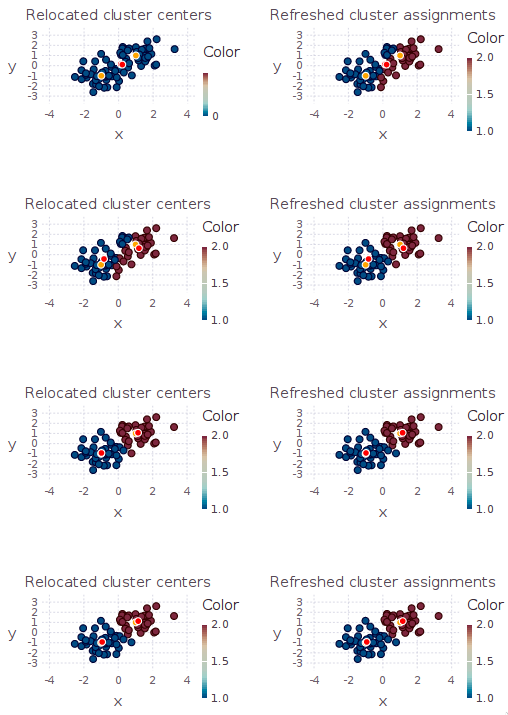
\includegraphics[width=300pt]{8_2}
  \caption{Clustering with k-means}
\end{figure}
The red dots are the true means, that the data was sampled from. The yellow dots
are the current estimates, that are converging towards the true means.

\section{Aufgabe 3}

\begin{minted}{julia}
using Gadfly, Distributions

# Number of iterations
iterations = 20

# Number of clusters
k = 2

# Color of clusters
colors = [color("red"), color("green")]

# True means
mus = [[-1, -1] [1, 1]]
# Random cluster centers
#mus = rand(2, k)

# Sample test data from the clusters
sigma2 = 1 / 2
Sigma = sigma2 * eye(2, 2)
numPoints = 40
data = [rand(MvNormal(float(mus[:, i]), Sigma), numPoints) for i = 1:size(mus, 2)]

# Make it a D*n matrix
data = hcat(data...)

set_default_plot_size(14cm, (iterations * 7cm))

function plotEllipsoid(mu, Sigma, c)
    # Plot a covariance matrix as an ellipsoid
    #
    # The ellipsoid is the distorted unit circle, but rescaled with it's largest eigenvalue.
    #
    # Returns a plot layer
    steps = 40
    circle = hcat([[cos(i), sin(i)] for i = linrange(0, 2 * pi, steps)]...)
    ellipse = (1 / eigmax(Sigma)) * Sigma * circle
    translated = ellipse .+ mu

    layer(x = translated[1, :], y = translated[2, :], Geom.path, Theme(default_color=c))
end

function plotEM(X, Mus, Sigmas, pis, taus; title="")
    # Plot all relevant state of the EM algorithm
    MusLayers = [layer(x = [Mus[1, i]], y = [Mus[2, i]], Geom.point, Theme(default_color=colors[i])) for i = 1:size(Mus, 2)]
    TrueMusLayer = layer(x = mus[1, :], y = mus[2, :], Geom.point, Theme(default_color=color("orange")))

    labels = taus[2, :]
    XLayer = layer(x = X[1, :], y = X[2, :], color=labels, Geom.point)

    layers = [MusLayers..., TrueMusLayer, XLayer]
    ellipsoids = [plotEllipsoid(Mus[:, i], Sigmas[i], colors[i]) for i = 1:size(Sigmas, 1)]
    layers = [ellipsoids..., layers...]

    plot(layers, Guide.title(title), Scale.ContinuousColorScale(Scale.lab_gradient(colors...)))
end

function emUpdateAssignments(X, k, mus, Sigmas, pis)
    # X - D*k matrix of data points
    # k - Number of models
    # mus - Means of the models
    # Sigmas - Covariances of the models
    # pis - Proportions of the models
    #
    # Returns a k*n matrix, where the columns are tau_i
    distributions = [MvNormal(float(mus[:, i]), Sigmas[i]) for i = 1:k]
    tau(x) = begin
        # Regularization constant (denominator)
        r = sum([pis[i] * pdf(distributions[i], x) for i = 1:k])

        (1 / r) * [pis[i] * pdf(distributions[i], x) for i = 1:k]
    end

    float(hcat([tau(X[:, i]) for i = 1:size(X, 2)]...))
end

function emUpdateMeans(X, taus)
    (X * taus') ./ (taus * ones(size(X, 2), 1))'
end

function emUpdateCovariances(X, k, taus, mus)
    tauSums = taus * ones(size(X, 2), 1)

    update(Taus, mu) = begin
        sum([Taus[i] * (X[:, i] - mu) * (X[:, i] - mu)' for i = 1:size(X, 2)])
    end

    [update(taus[i, :], mus[:, i]) / tauSums[i] for i = 1:k]
end

function emUpdateProportions(X, taus)
    ((1 / size(X, 2)) * (taus * ones(size(X, 2), 1)))'
end

function EM(X, k, iters)
    # X - D*n matrix of data points
    # k - Number of clusters
    # iters - Number of iterations

    # Random initial parameters
    mus = rand(2, k)
    Sigmas = [eye(2) for i = 1:k]
    pis = rand(1, k)
    taus = zeros(k, size(X, 2))

    iteration(i) = begin
        plot1 = plotEM(X, mus, Sigmas, pis, taus, title="Relocated cluster centers")
        taus = emUpdateAssignments(X, k, mus, Sigmas, pis)
        plot2 = plotEM(X, mus, Sigmas, pis, taus, title="Refreshed cluster assignments")
        mus = emUpdateMeans(X, taus)
        Sigmas = emUpdateCovariances(X, k, taus, mus)
        pis = emUpdateProportions(X, taus)

        hstack(plot1, plot2)
    end

    plots = map(iteration, 1:iters)

    vstack(plots...)
end

EM(data, k, iterations)
\end{minted}
The EM algorithm (empirically) converges slower than k-means. It took me several
tries to get a sample, that EM converged on in the first 20 iterations.
\begin{figure}[ht]
  \centering
  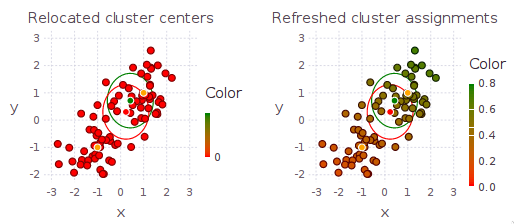
\includegraphics[width=300pt]{8_3_1}
  \caption{Initial setup (the coloring in the left graph is meaningless)}
\end{figure}
\begin{figure}[ht]
  \centering
  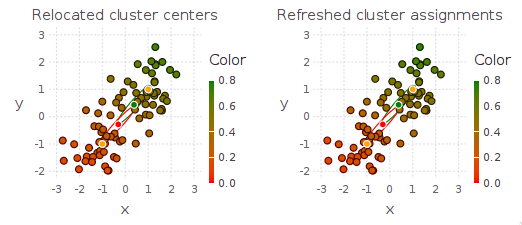
\includegraphics[width=300pt]{8_3_2}
  \caption{2. iteration}
\end{figure}
\begin{figure}[ht]
  \centering
  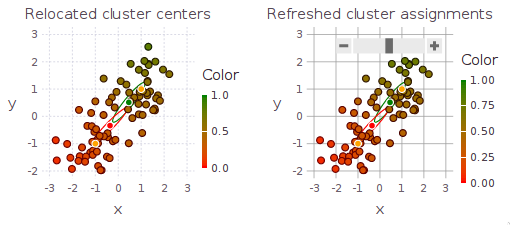
\includegraphics[width=300pt]{8_3_3}
  \caption{5. iteration}
\end{figure}
\begin{figure}[ht]
  \centering
  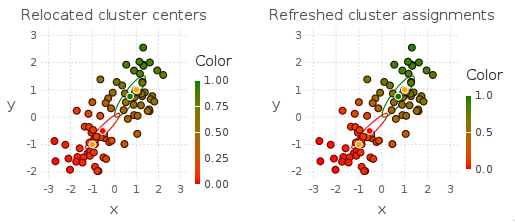
\includegraphics[width=300pt]{8_3_4}
  \caption{10. iteration (The clusters are separating fast at this stage)}
\end{figure}
\begin{figure}[ht]
  \centering
  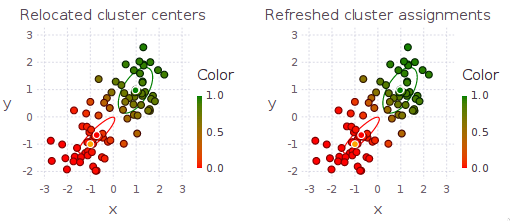
\includegraphics[width=300pt]{8_3_5}
  \caption{13. iteration}
\end{figure}
\begin{figure}[ht]
  \centering
  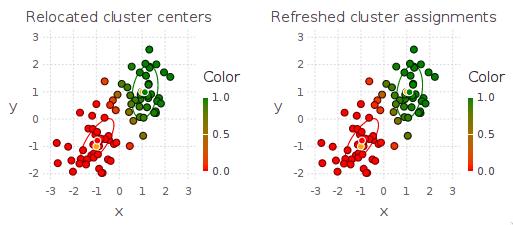
\includegraphics[width=300pt]{8_3_6}
  \caption{17. iteration (Converged)}
\end{figure}

\end{document}